\section{Búsquedas de Artículos}
Originalmente la base de datos contenía unos 7777 papers, de los cuáles se tuvo que hacer una depuración de los mismo, ya que había papers que no tenían ningún autor asociado. Luego de la depuración quedaron 4937 que cumplen los requisitos para la búsqueda de las soluciones.
\subsection{Soluciones repetidas}
En las primeras pruebas pruebas de la implementación de las búsquedas se usaron todos los artículos. Se observaron que todas las soluciones tenían un alto valor en su función objetivo, al analizar en detalle las soluciones y los artículos de cada uno de los bundles se encotró que muchos de esos artículos tenían un solo elemento de temática en su topicProfile.\\
Esto ocasionaba que para los difrentes $\gamma$ que se probara el algoritmo HAC, éste generaba soluciones practicamente idénticas ya que los valores inter e intra alcanzaban valores cercanos al máximo. Ocasionando la pérdida de variedad en las soluciones. A fines de comparar las implementaciones generadas y obtener resultados más interesantes, se decidió no tener en cuenta a los artículos con un solo topicProfile.\\
\subsection{Soluciones con bundles unitarios}
En las pruebas en las que se intenta priorizar el inter, se observó que se generaban muchos bundles unitarios o de dos elementos a causa de que existían artículos sin topicProfile por lo se decidió no tenerlos en cuenta. Otra causa que se identificó fue que en la generación de bundles de HAC, no estaba seleccionando bien los bundles ya que siempre prioriza la similitud inter, por ejemplo: Existen 5 articulos del topico 'METHODOLOGIES' donde su distribution > 0.7. Estos 5 articulos pertenecen a 3 venues distintos, venue A para el articulo 1, venue B para el articulo 2 y venue C para el resto. El jerarquico genera 3 bundles: uno con el articulo 1 con uno del venue C, otro con el articulo 2 con otro del venue C y por ultimo un bundle con el restante articulo del venue C.\\
Luego uno de estos bundles (el de mayor intra) es seleccionado para la solución ya que es el unico que contiene el topic 'METHODOLOGIES'  En este caso se podría haber generado un bundle que contenga articulos de los 3 bundles. Para mejorar el intra. Una posible solución que se elaboró, pero no se implementó, para corregir este problema fue intentar realizar una búsqueda sobre los bundles que no superaron el presupuesto e intercambiar con elementos de otros en caso que se mejore su similitud intra.
\subsection{Comparando}
Para comparar la calidad de las distintas soluciones, además del valor objetivo se compara con la cantidad de elementos iguales en toda la solución y la cantidad igual de elementos para cada bundle. De esta manera se observa que tan \textquotedblleft parecidas\textquotedblright son las soluciones y con más detalle que tan \textquotedblleft parecidos\textquotedblright son los bundles.\\ 
Entre los diferentes algoritmos buscamos la cantidad de elementos iguales en cada una de las soluciones y también la cantidad de elementos iguales por bundle. Se generaron soluciones con las siguientes características:\\
\Solucion
{}
{simple}
{\texttt{SingleHAC}, \texttt{EfficientHAC} y \texttt{Greedy}}
{$\in$ $(0,1; 0,3; 0,5; 0,7; 0,9)$}
{10}
{5}
Como primera observación podemos ver la cantidad de bundles que se generan para cada algoritmo de 
producción:\\
\begin{table}[h]
  \centering
  \resizebox{0.5\textwidth}{!} {
    \begin{tabular}{|lc|}
    \hline
    Algoritmo & Bundles Generados \\
    \hline
    SingleHAC & $2378$ \\
    EfficientHAC & $2378$ \\
    Greedy & $10$ \\
    \hline
    \end{tabular}
  }
    \caption {Cantidad de bundles generados antes de la selección final}
\end{table}

En los siguientes gráficos se visualiza los resultados obtenidos para $\gamma$ 0.1 y 0.9. Cada 
nodo representa un bundle y los ejes el valor de la similitud entre cada uno de ellos. La línea más 
gruesa indica un mayor grado de similitud. En cuanto a los vértices al acercarse al azul el valor 
de la intra es menor y al rojo mayor.

\begin{figure}[H]
  \centering
    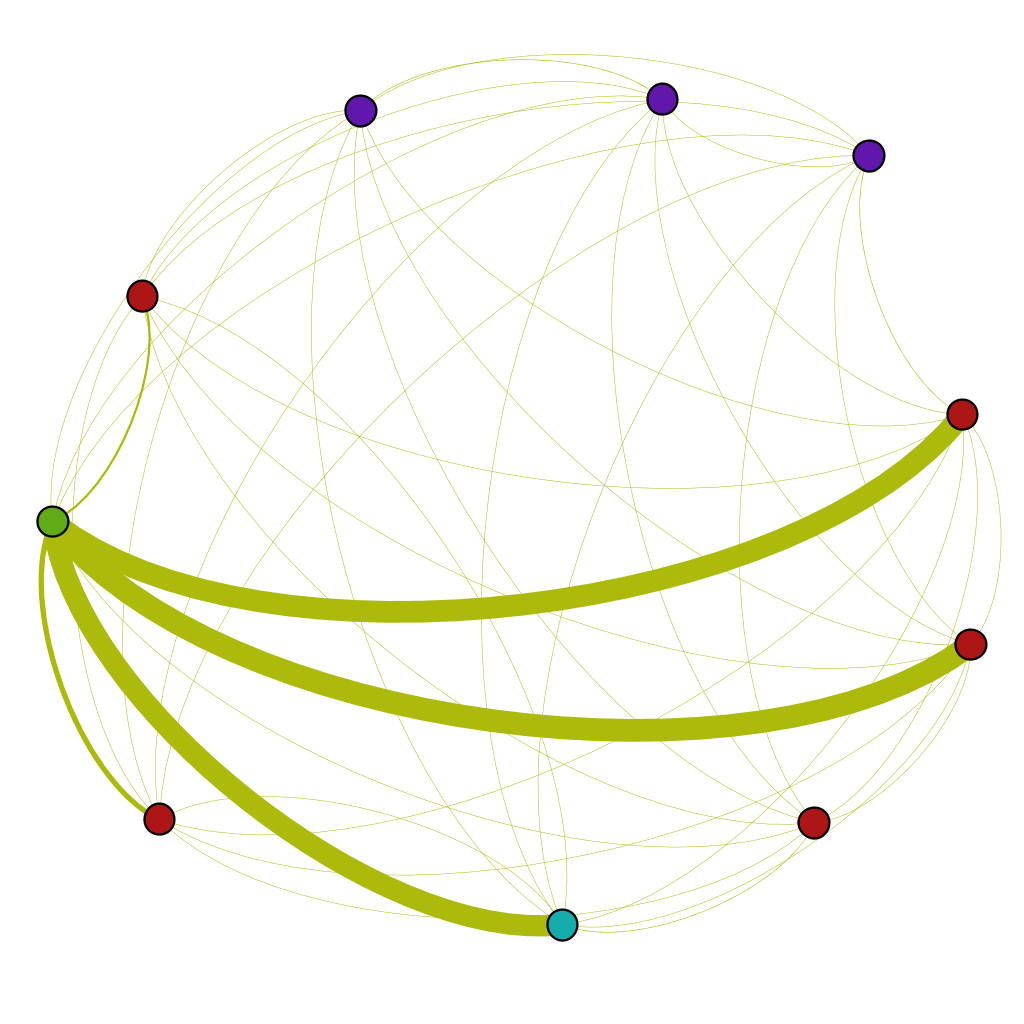
\includegraphics[width=0.5\textwidth]{resultados/papers/intra_inter/hac01.png}
  \caption{Relación entre bundles para $\gamma$ = $0.1$ y algoritmo SingleHAC}
  \label{res:img-papers-gamma01-hac}
\end{figure}

\begin{figure}[H]
  \centering
    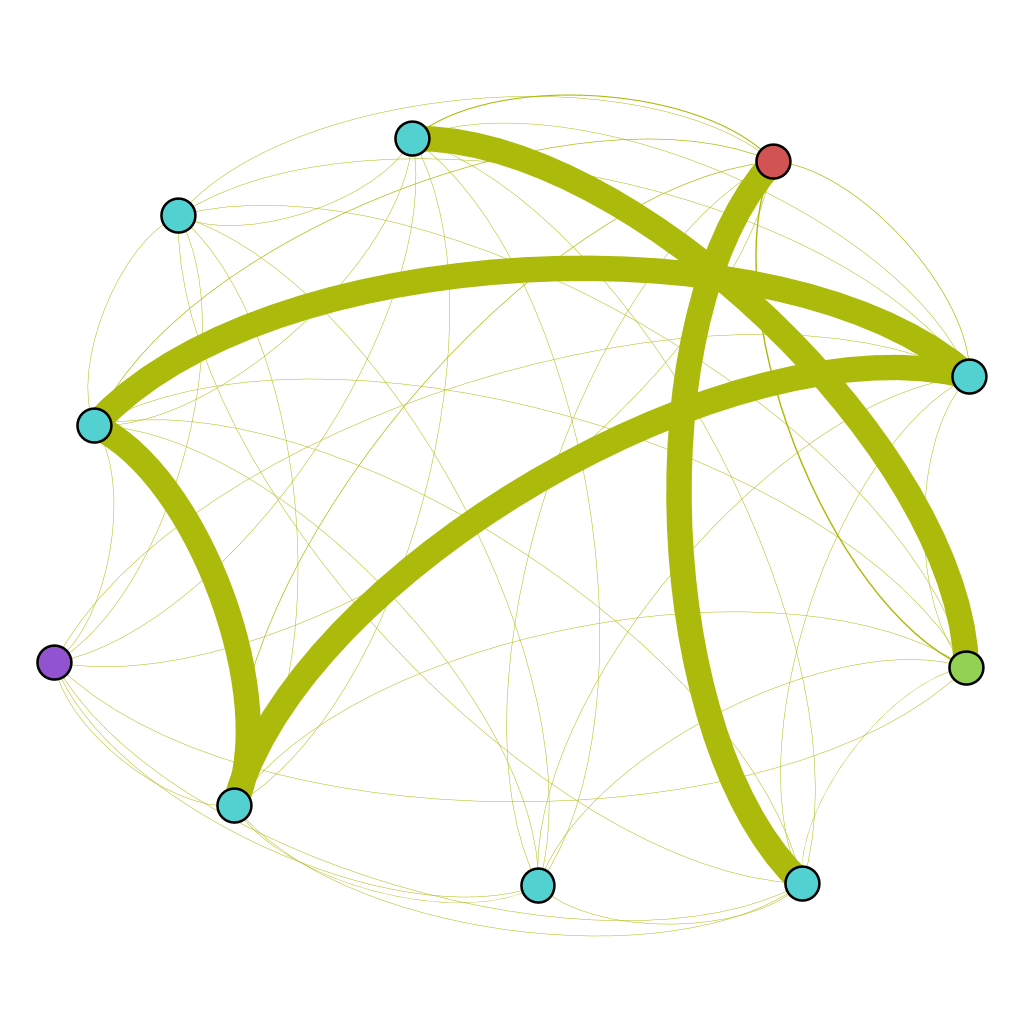
\includegraphics[width=0.5\textwidth]{resultados/papers/intra_inter/hac09.png}
  \caption{Relación entre bundles para $\gamma$ = $0.9$ y algoritmo SingleHAC}
  \label{res:img-papers-gamma09-hac}
\end{figure}

\begin{figure}[H]
  \centering
    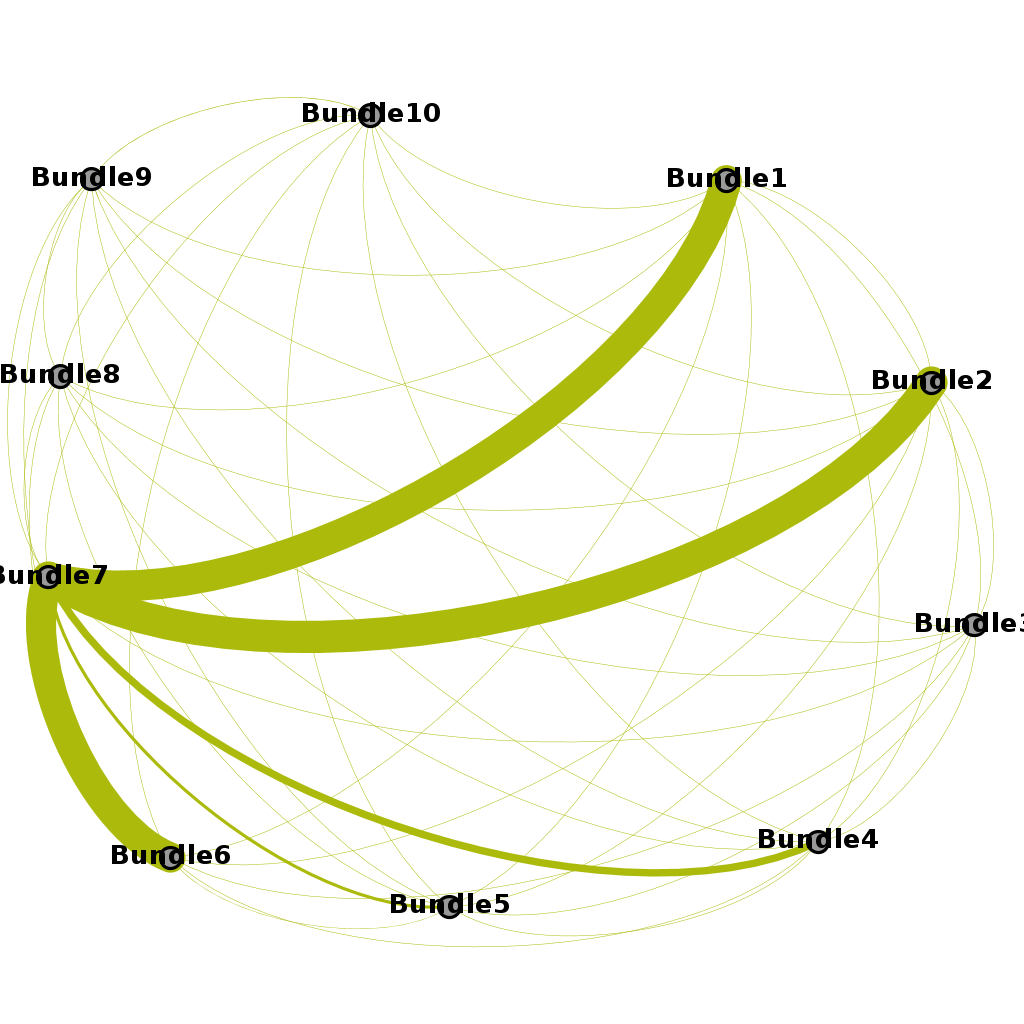
\includegraphics[width=0.5\textwidth]{resultados/papers/intra_inter/effhac01.png}
  \caption{Relación entre bundles para $\gamma$ = $0.1$ y algoritmo EfficientHAC}
  \label{res:img-papers-gamma01-effhac}
\end{figure}

\begin{figure}[H]
  \centering
    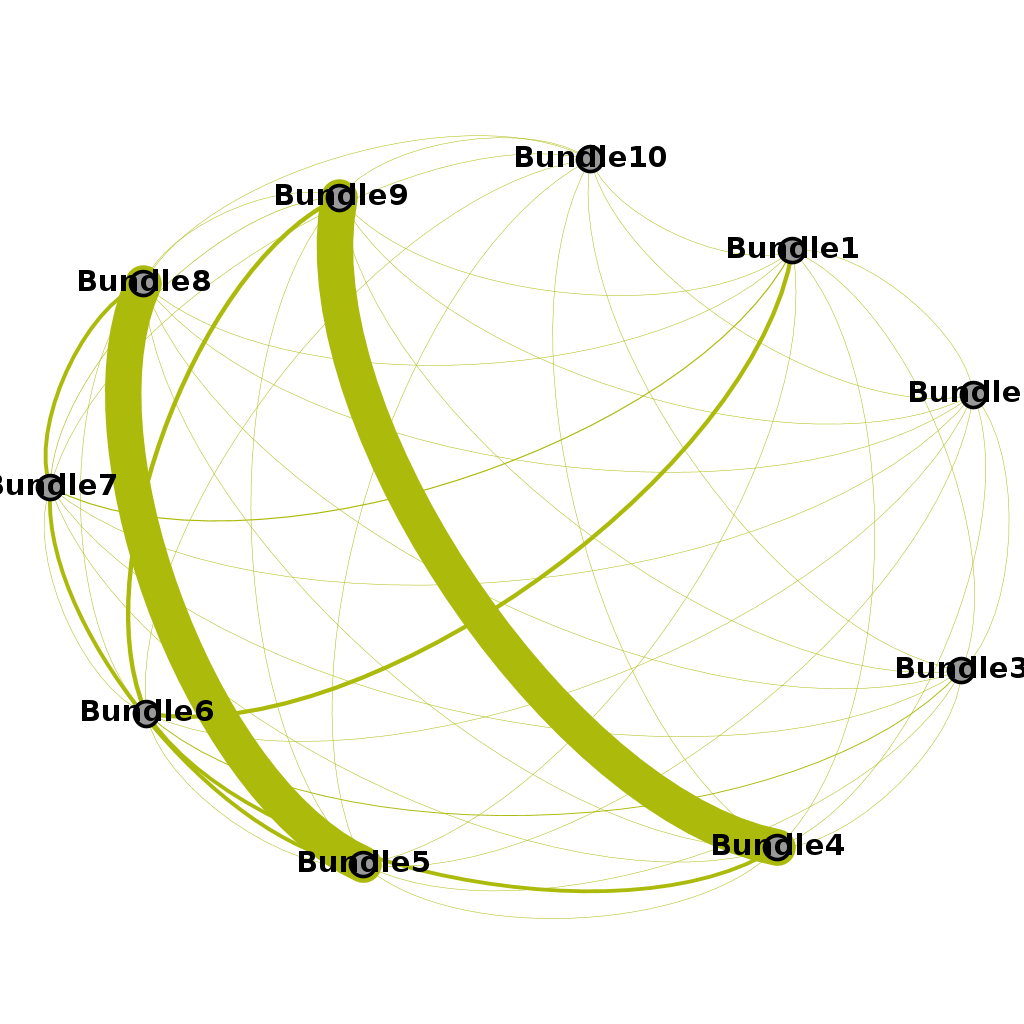
\includegraphics[width=0.5\textwidth]{resultados/papers/intra_inter/effhac09.png}
  \caption{Relación entre bundles para $\gamma$ = $0.9$ y algoritmo EfficientHAC}
  \label{res:img-papers-gamma09-effhac}
\end{figure}

\begin{figure}[H]
  \centering	
    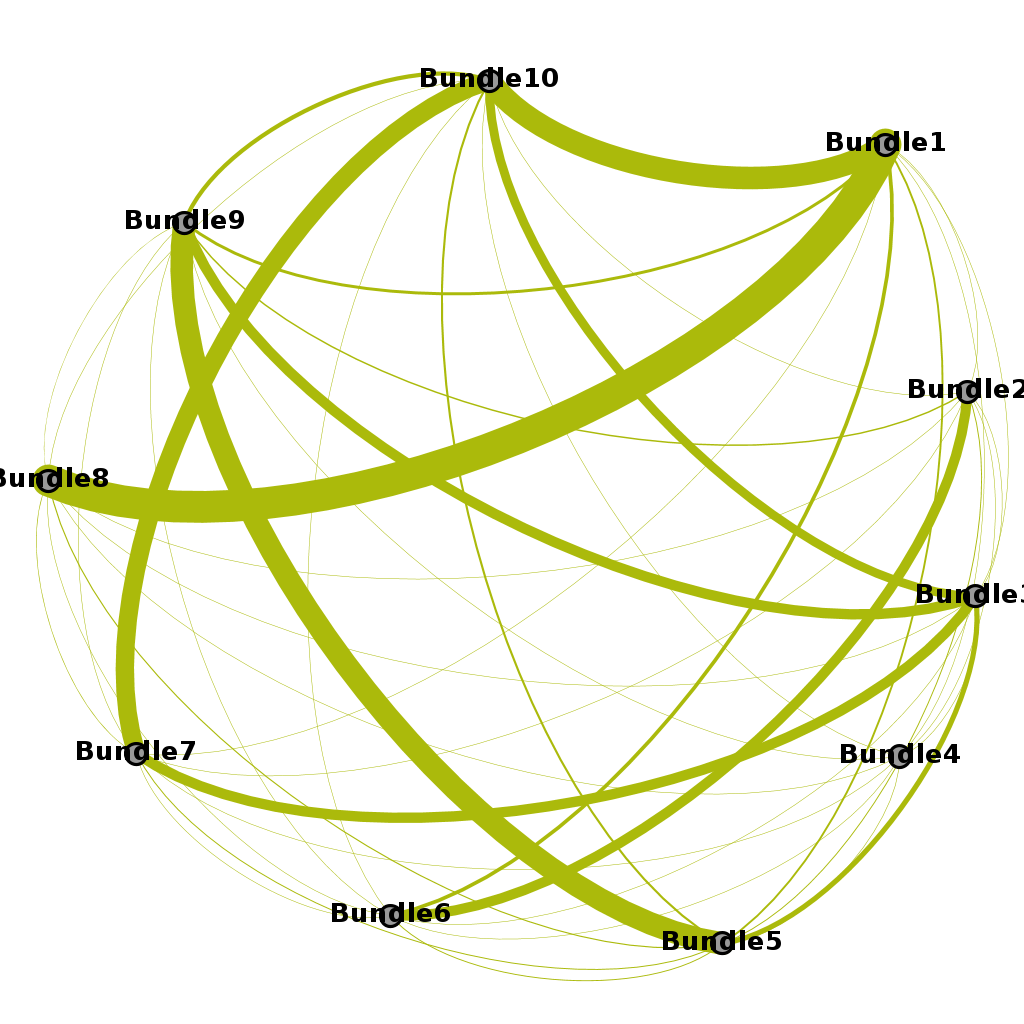
\includegraphics[width=0.5\textwidth]{resultados/papers/intra_inter/greedy01.png}
  \caption{Relación entre bundles para $\gamma$ = $0.1$ y algoritmo Greedy}
  \label{res:img-papers-gamma01-greedy}
\end{figure}

\begin{figure}[H]
  \centering
    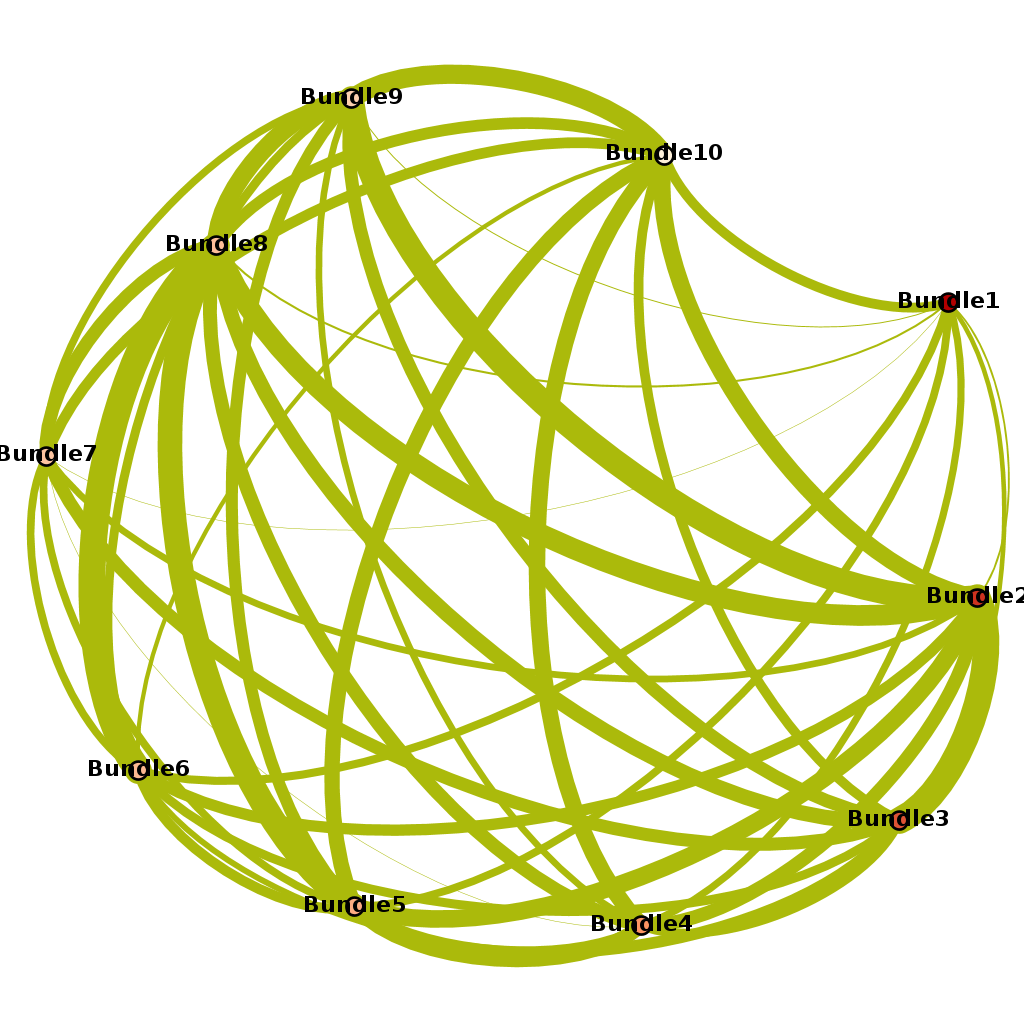
\includegraphics[width=0.5\textwidth]{resultados/papers/intra_inter/greedy09.png}
  \caption{Relación entre bundles para $\gamma$ = $0.9$ y algoritmo Greedy}
  \label{res:img-papers-gamma09-greedy}
\end{figure}

\section{Autores}
Se generaron soluciones con las siguientes características:\\
\Solucion
{}
{simple y proporcional}
{\texttt{SingleHAC}, \texttt{EfficientHAC} y \texttt{Greedy}}
{$\in$ $(0,1; 0,3; 0,5; 0,7; 0,9)$}
{10}
{5}

En los siguientes gráficos se visualiza los resultados obtenidos para $\gamma$ 0.1 y 0.9. Cada 
nodo representa un bundle y los ejes el valor de la similitud entre cada uno de ellos. La línea más 
gruesa indica un mayor grado de similitud. En cuanto a los vértices al acercarse al azul el valor 
de la intra es menor y al rojo mayor.

\begin{figure}[H]
  \centering
    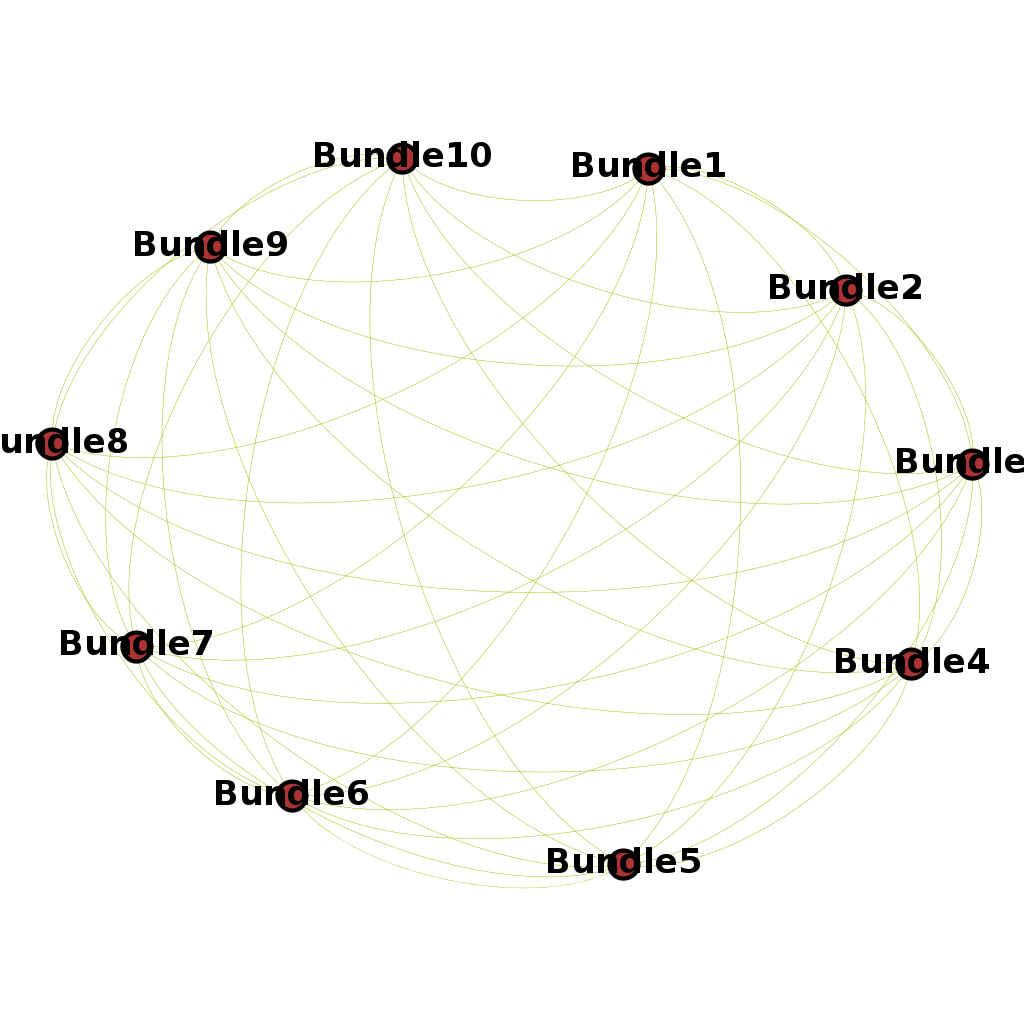
\includegraphics[width=0.5\textwidth]{resultados/authors/intra_inter/hac01.png}
  \caption{Relación entre bundles para $\gamma$ = $0.1$ y algoritmo SingleHAC, selección simple}
  \label{res:img-authors-gamma01-hac}
\end{figure}

\begin{figure}[H]
  \centering
    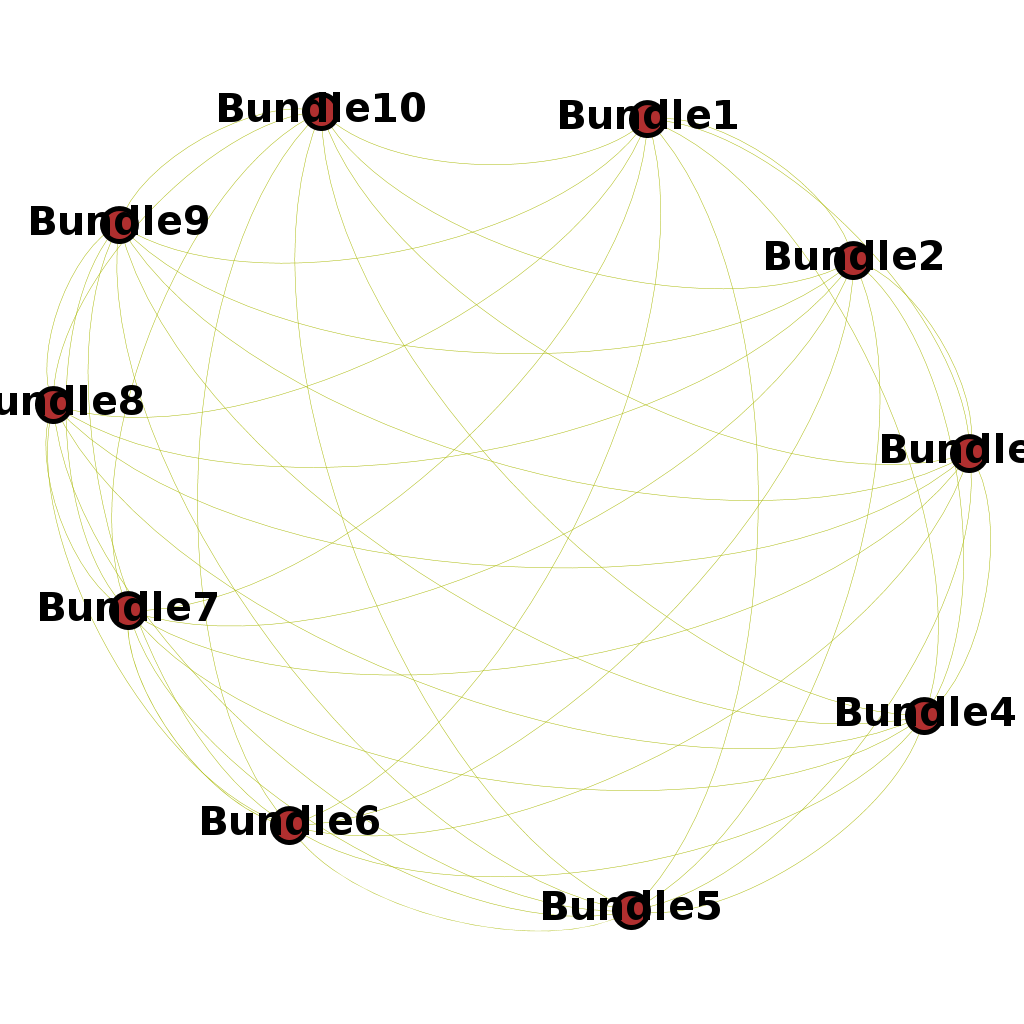
\includegraphics[width=0.5\textwidth]{resultados/authors/intra_inter/hac09.png}
  \caption{Relación entre bundles para $\gamma$ = $0.9$ y algoritmo SingleHAC, selección simple}
  \label{res:img-authors-gamma09-hac}
\end{figure}

\begin{figure}[H]
  \centering
    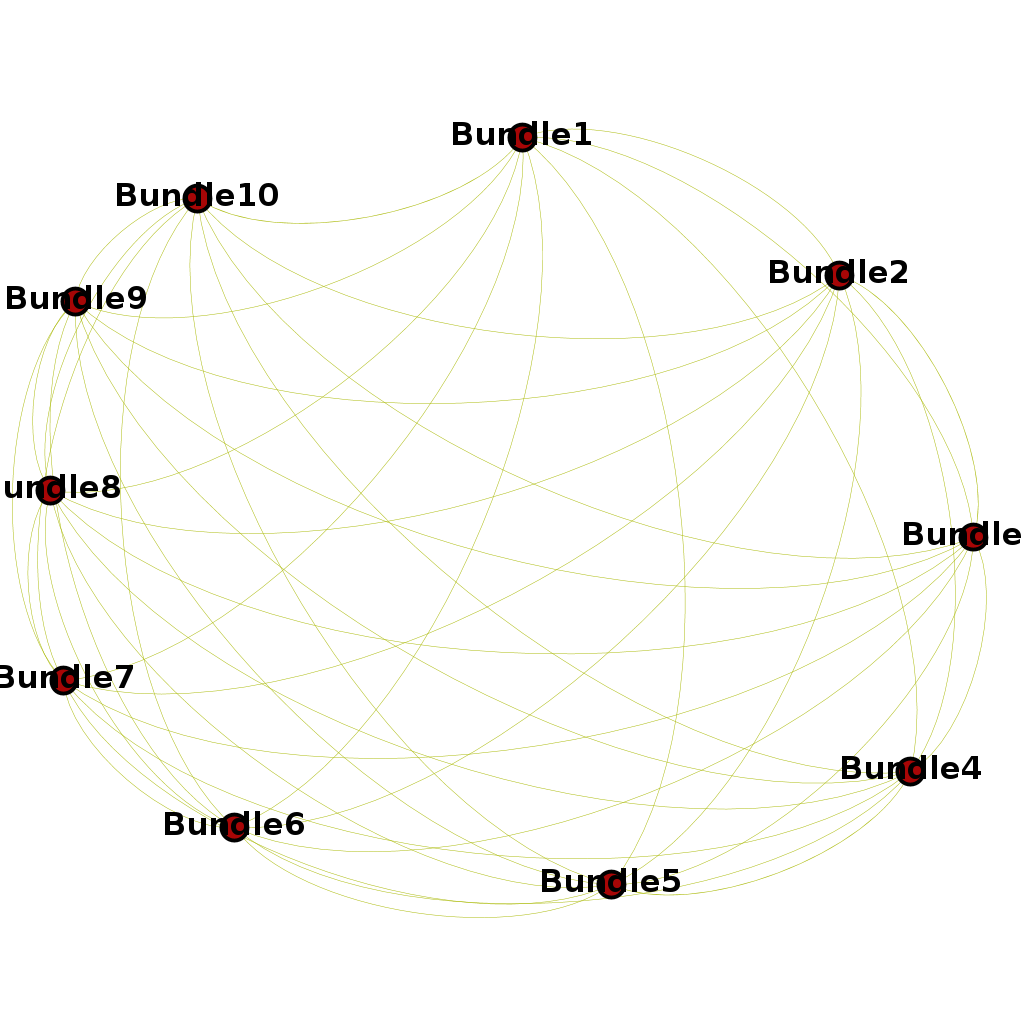
\includegraphics[width=0.5\textwidth]{resultados/authors/intra_inter/effhac01.png}
  \caption{Relación entre bundles para $\gamma$ = $0.1$ y algoritmo EfficientHAC, selección simple}
  \label{res:img-authors-gamma01-effhac}
\end{figure}

\begin{figure}[H]
  \centering
    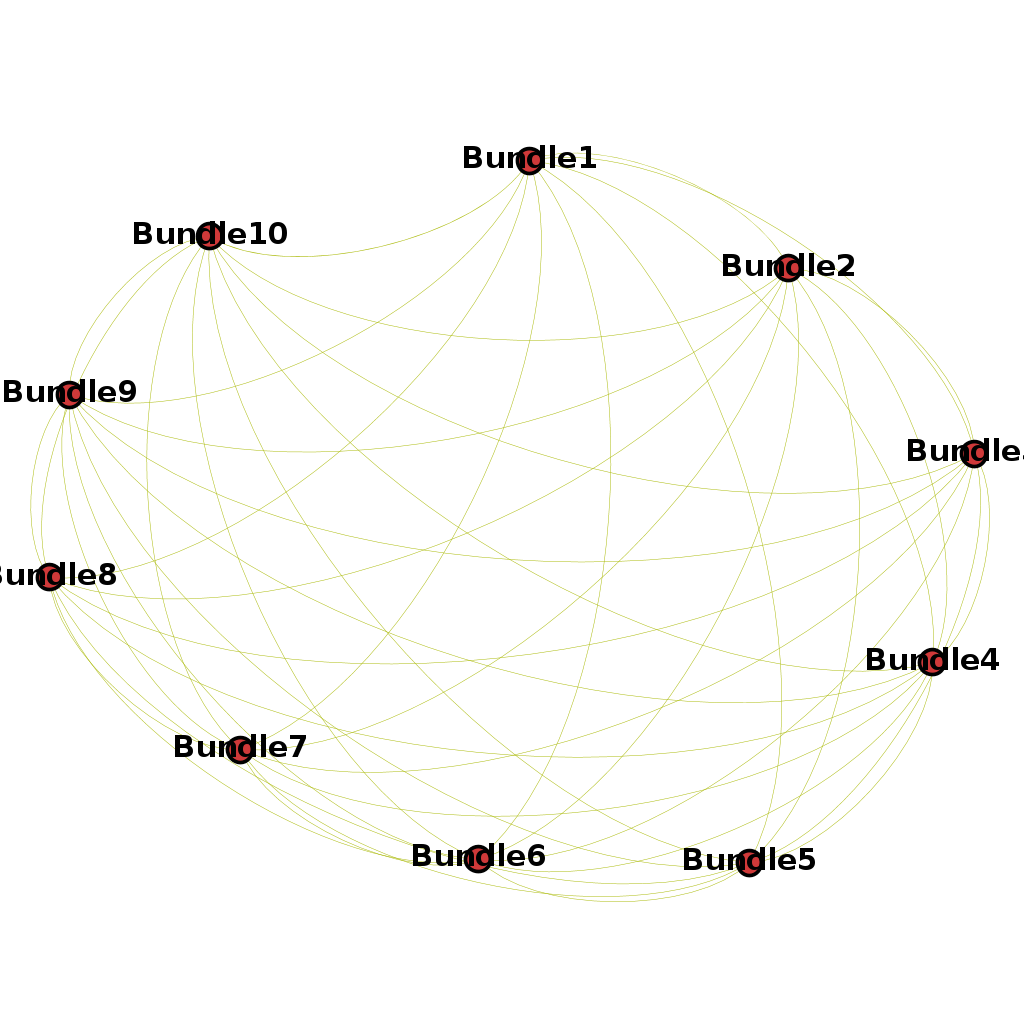
\includegraphics[width=0.5\textwidth]{resultados/authors/intra_inter/effhac09.png}
  \caption{Relación entre bundles para $\gamma$ = $0.9$ y algoritmo EfficientHAC, selección simple}
  \label{res:img-authors-gamma09-effhac}
\end{figure}

\begin{figure}[H]
  \centering
    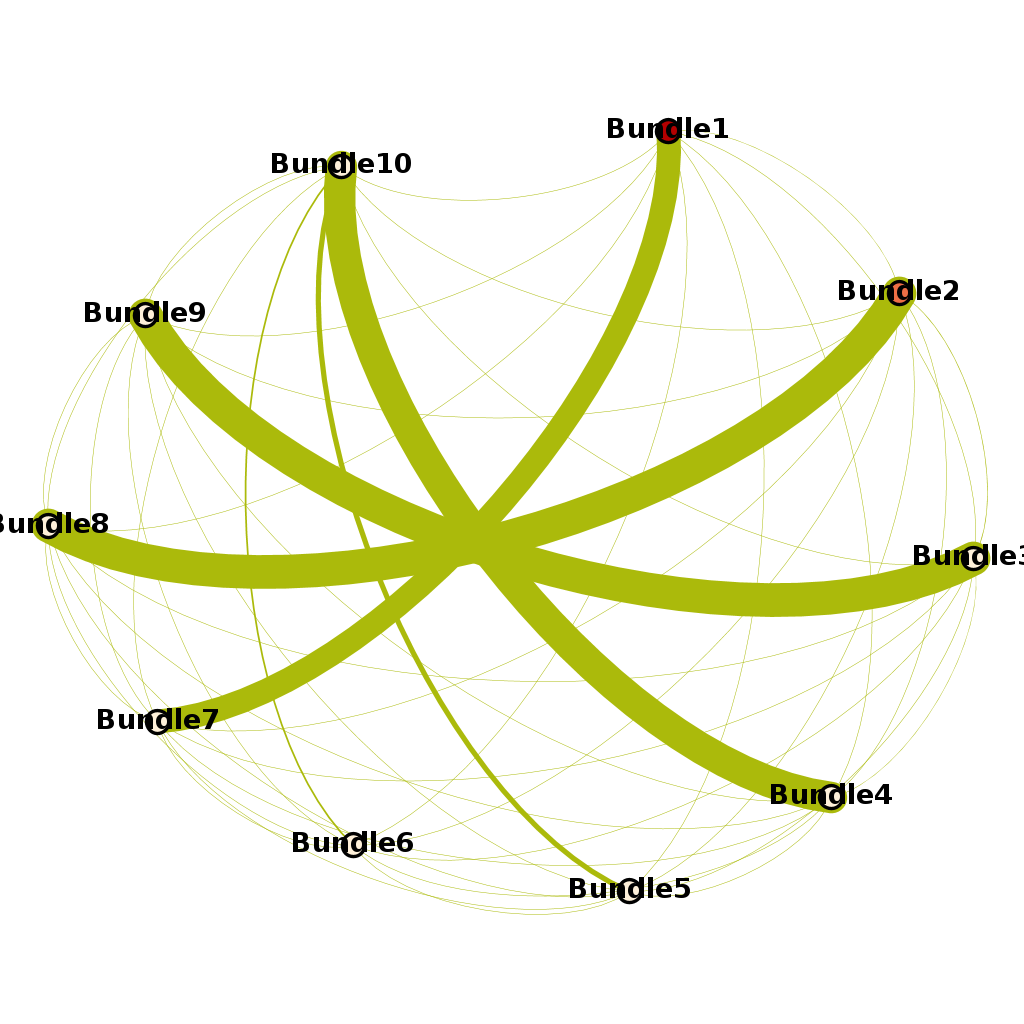
\includegraphics[width=0.5\textwidth]{resultados/authors/intra_inter/greedy01.png}
  \caption{Relación entre bundles para $\gamma$ = $0.1$ y algoritmo Greedy}
  \label{res:img-authors-gamma01-greedy}
\end{figure}

\begin{figure}[H]
  \centering
    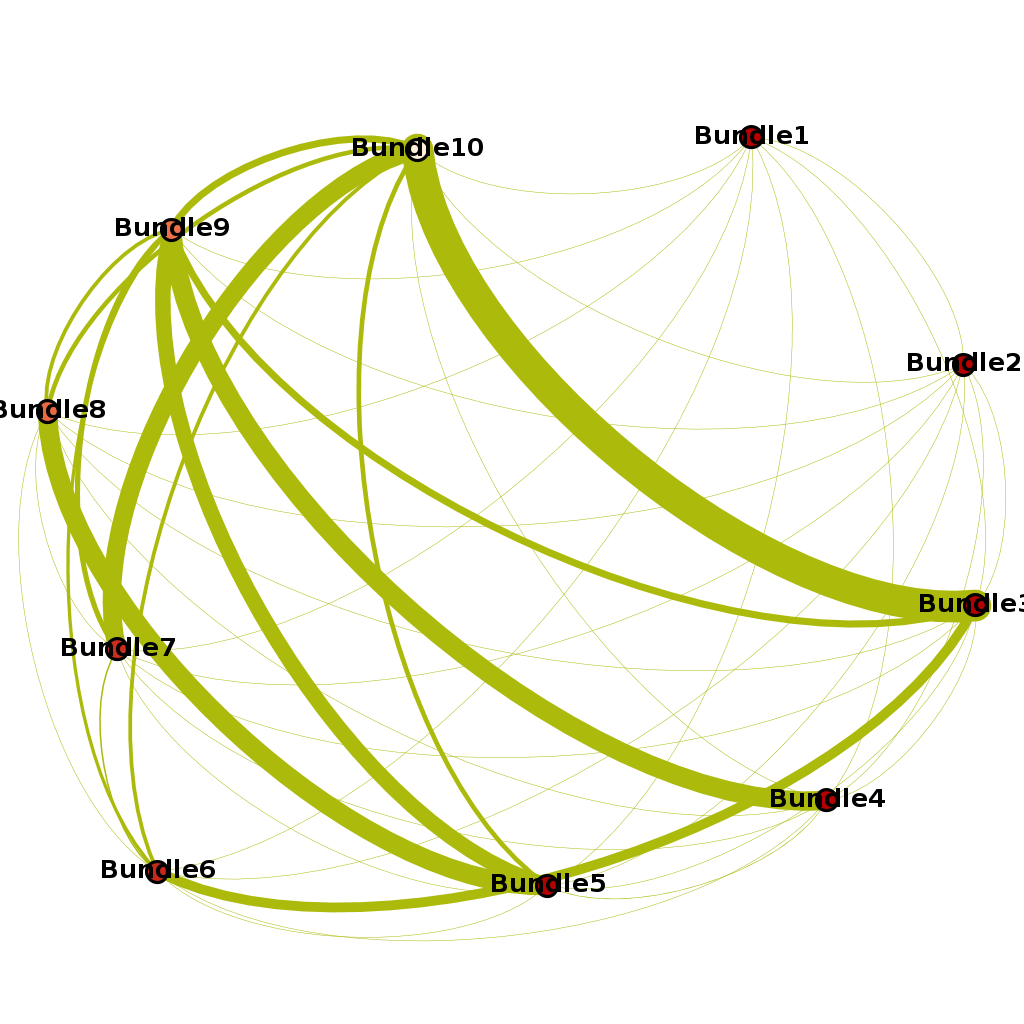
\includegraphics[width=0.5\textwidth]{resultados/authors/intra_inter/greedy09.png}
  \caption{Relación entre bundles para $\gamma$ = $0.9$ y algoritmo Greedy}
  \label{res:img-authors-gamma09-greedy}
\end{figure}

Tanto para las soluciones generadas por \texttt{SingleHAC} como por \texttt{EfficientHAC} y con 
cualquier estrategia de selección, todas las soluciones formaron los mismos bundles a pesar de la 
variación del parámetro $\gamma$. Esto se puede ver en los gráficos ya que todos los bundles 
tienen el mayor valor posible para la similitud intra y ningún bundle tiene relación con el 
resto.\\
En parte se debe a que existen $40000$ relaciones de similitud con valor uno. Con la 
heurística Produce and Choose, al momento de producir no se tiene en cuenta el $\gamma$ por lo tanto 
para todos los $\gamma$ en la etapa de producción se producen los mismos bundles.\\
Se realizaron otras búsquedas de soluciones, excluyendo a cinco de los autores que se encuentran 
presentes en todas las soluciones. Pero aún de esta manera en los nuevos resultados obtenidos se 
repite el mismo comportamiento que antes.\\
Además como veremos en \ref{conc:compDifAlgo} los resultados para las ejecuciones con los 
algoritmos jerárquicos se encuentran en los óptimos.
%Por otro lado todas las soluciones generadas por el algoritmo \texttt{HAC} prácticamente no 
%comparten bundles similares con las demás soluciones, ni siquiera autores similares en toda la 
%solución.

\section{Búsqueda con perfil específico}
En una primera aproximación para realizar esta búsqueda solo se modifico la generación de bundles, 
lo cuál, si bien generó resultados diferentes al algoritmo original, no se veía reflejado en los 
resultados las temáticas de los bundles con la elegida para la búsqueda.\\
A partir de ello se decidió modificar también la selección de los bundles para intentar obtener 
bundles relevantes con el perfil elegido.\\
A continuación mostramos la temáticas obtenidas para una búsqueda con un perfil específico de 
ALGORITHM = 50 \%, DISTRIBUTED SYSTEMS = 25 \% y KNOWLEDGE ENGINEERING = 25 \% para la ejecución 
del algoritmo SingleHAC con $\gamma$ = 0.1 y $\gamma$ = 0.9.
\begin{figure}[H]
  \centering
    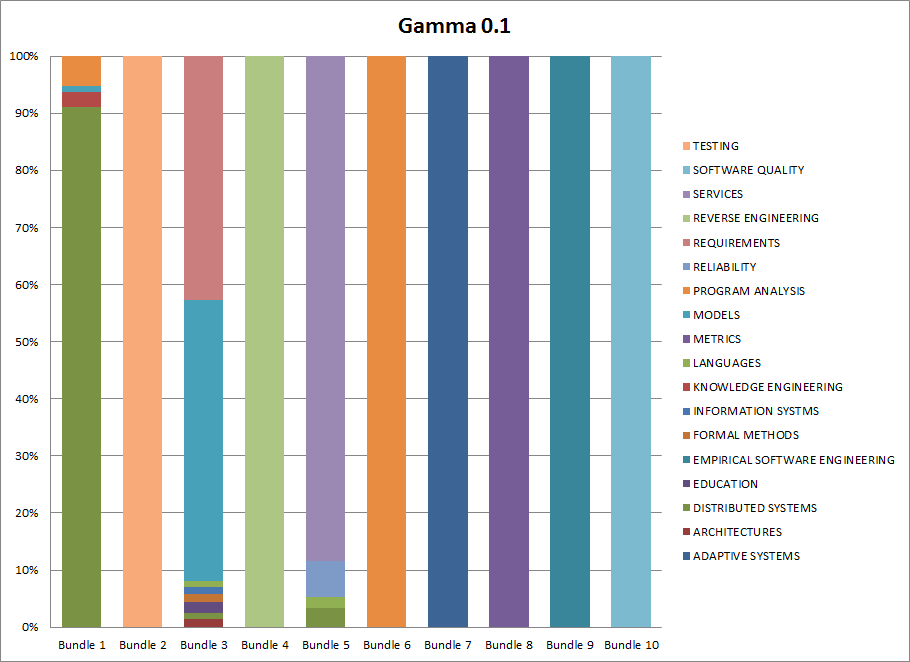
\includegraphics[width=\textwidth]{resultados/papers/intra_inter/grafico_gamm01.png}
  \caption{$\gamma$ = 0.1}
  \label{res:img-gamma01-especifico}
\end{figure}

\begin{figure}[H]
  \centering
    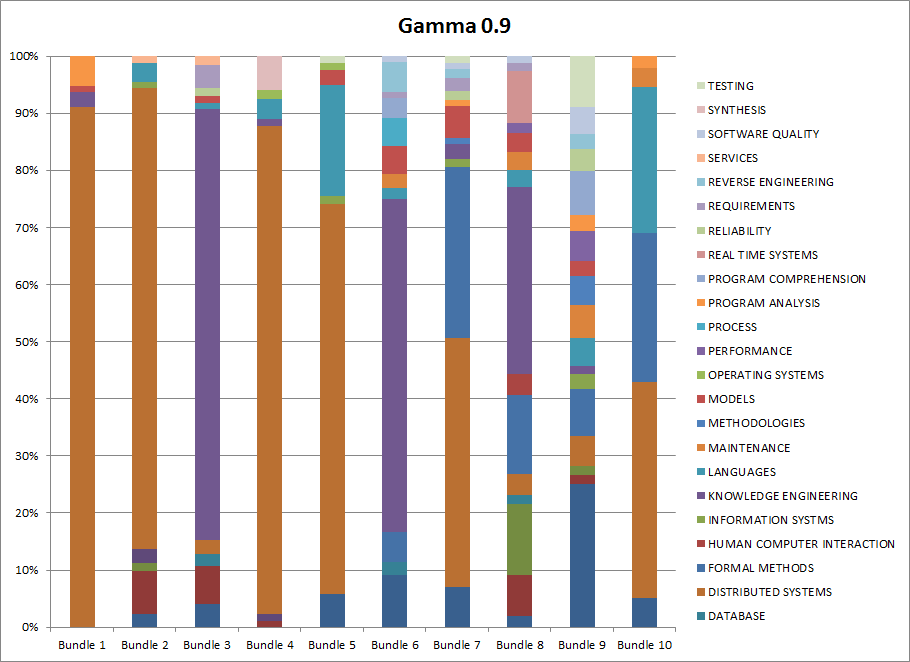
\includegraphics[width=\textwidth]{resultados/papers/intra_inter/grafico_gamm09.png}
  \caption{$\gamma$ = 0.9}
  \label{res:img-gamma09-especifico}
\end{figure}